\section{Taught Poses and Robot Motion}
The taught poses, robot feedback, and gripper settings below belong to physical execution. Simulation uses the separate MoveIt and grasp-constraint workflow in Section~\ref{sec:simulation}.


\subsection{Recording the physical pickup and placement poses}

The fixed cells allowed us to use a small set of taught robot poses. After vision selected a cell and a sorting group, the worker loaded its pickup poses and the correct destination poses. This reduced the need to estimate a new three-dimensional grasp point from each image. It also made the limits clear: the camera, robot base, grid sheet, and gripper had to stay in their calibrated positions, and each object had to be placed near its cell center.\src{teaching,motion}

The physical recorder guided the operator through 17 named poses. It stored six joint angles and the tool center point (TCP) position and orientation for each pose. The source approach poses were taught above the objects; the grasp poses placed the fingers at the required pickup height. Both destinations had an approach pose and a lower release pose. A shared safe pose linked the source and destination routes.\src{teaching}

\begin{table}[H]\tabstart
\caption{The 17 named poses used by the physical task}
\begin{tabularx}{\textwidth}{@{}L{1.7cm}Y C{1cm}@{}}
\toprule Location & Pose names & Count\\\midrule
Shared & \file{safe} & 1\\
Grid 1 & \file{grid_1_approach}, \file{grid_1_grasp} & 2\\
Grid 2 & \file{grid_2_approach}, \file{grid_2_grasp} & 2\\
Grid 3 & \file{grid_3_approach}, \file{grid_3_grasp} & 2\\
Grid 4 & \file{grid_4_approach}, \file{grid_4_grasp} & 2\\
Grid 5 & \file{grid_5_approach}, \file{grid_5_grasp} & 2\\
Grid 6 & \file{grid_6_approach}, \file{grid_6_grasp} & 2\\
Left area & \file{left_approach}, \file{left_release} & 2\\
Right area & \file{right_approach}, \file{right_release} & 2\\\midrule
Total & One shared pose, twelve source poses, four destination poses & 17\\
\bottomrule
\end{tabularx}
\end{table}

The formal transfer code required a complete pose file and an active correction record covering all 17 points. It checked the angle limits and rejected invalid values before motion. The inherited simulation tools used RViz and the \file{q}/\file{qa}/\file{qb} keyframe method. They were useful for learning and checking motion ideas, while the physical Experiment 3 route used the named-pose recorder above. The two formats should not be treated as the same dataset.\src{teaching,motion,defense}

\subsection{Small joint steps and the transfer sequence}

The robot moved between taught joint targets using linear interpolation. Let $\mathbf q_0$ and $\mathbf q_1$ be two six-joint vectors, and let $\delta$ be the largest allowed command step. The program used
\begin{equation}
N=\max\!\left(1,\left\lceil\frac{\max_j|q_{1,j}-q_{0,j}|}{\delta}\right\rceil\right),
\qquad
\mathbf q_k=\mathbf q_0+\frac{k}{N}(\mathbf q_1-\mathbf q_0),\quad k=1,\ldots,N.
\end{equation}
Thus, no joint command changed by more than $\delta$ within one step. The final launch set $\delta=2^{\circ}$, a command interval of 0.20 s, and an SDK arm-speed value of 8. These are software settings; 8 is not a measured speed in degrees per second.\src{motion,integration}

The commands were sent in small steps, and feedback was checked at key poses. Joint interpolation did not guarantee a straight TCP path or impose a verified acceleration limit. We therefore relied on the taught layout, safe transition poses, and measured endpoint checks.\src{motion}

A transfer began at the safe pose with the gripper open. The arm moved above the selected cell, checked the open gripper, descended, and closed to the class-specific setting. After lifting, it checked the grip and returned through the safe pose. It then approached the selected destination, descended, released the object, lifted clear, and returned to safe. Figure~\ref{fig:motion-stages} shows three physical stages from the defense presentation.\src{motion,defense}

\begin{figure}[H]
\centering
\begin{subfigure}[t]{0.32\textwidth}
\centering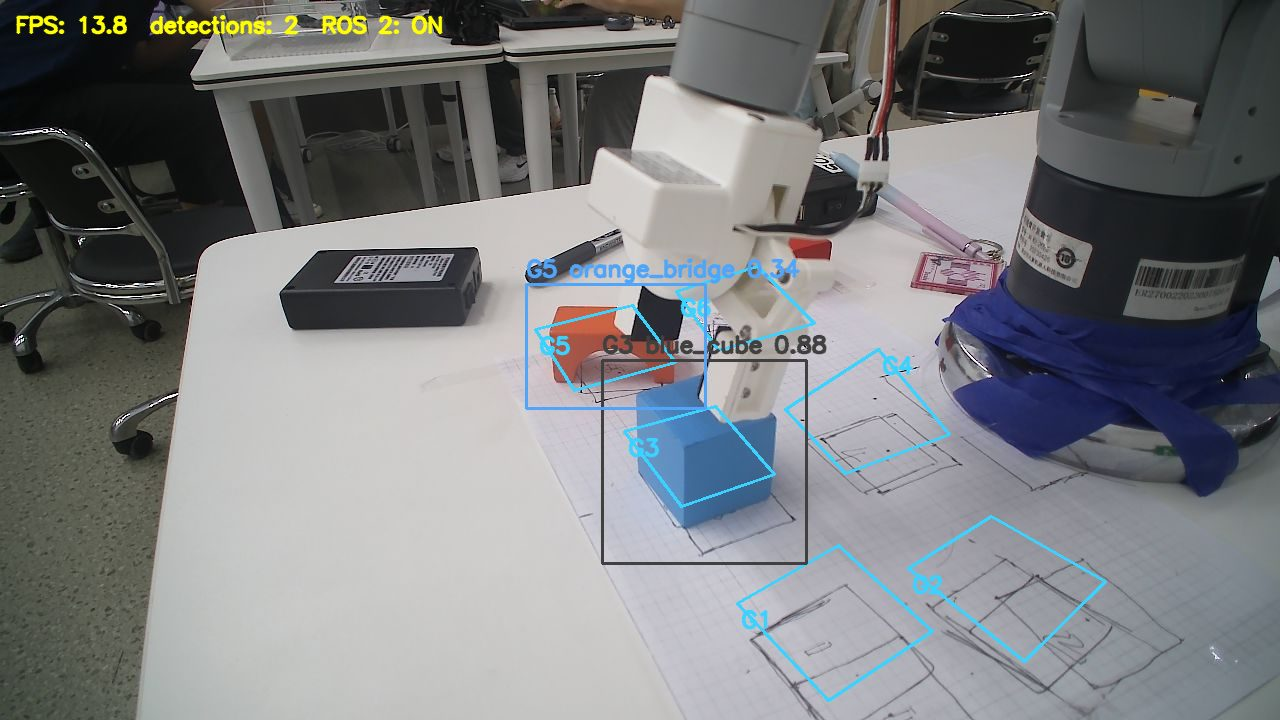
\includegraphics[width=\linewidth]{figures/approach.jpg}
\caption{Approach the source.}
\end{subfigure}\hfill
\begin{subfigure}[t]{0.32\textwidth}
\centering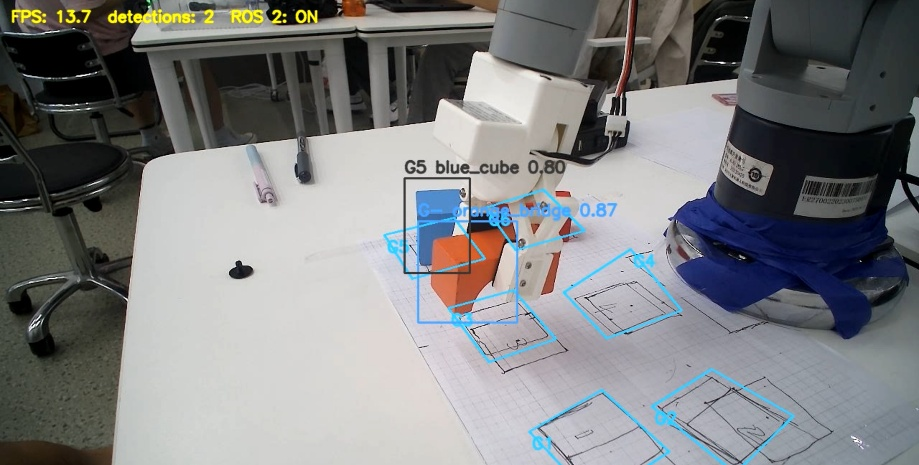
\includegraphics[width=\linewidth]{figures/grasp.jpg}
\caption{Descend and grasp.}
\end{subfigure}\hfill
\begin{subfigure}[t]{0.32\textwidth}
\centering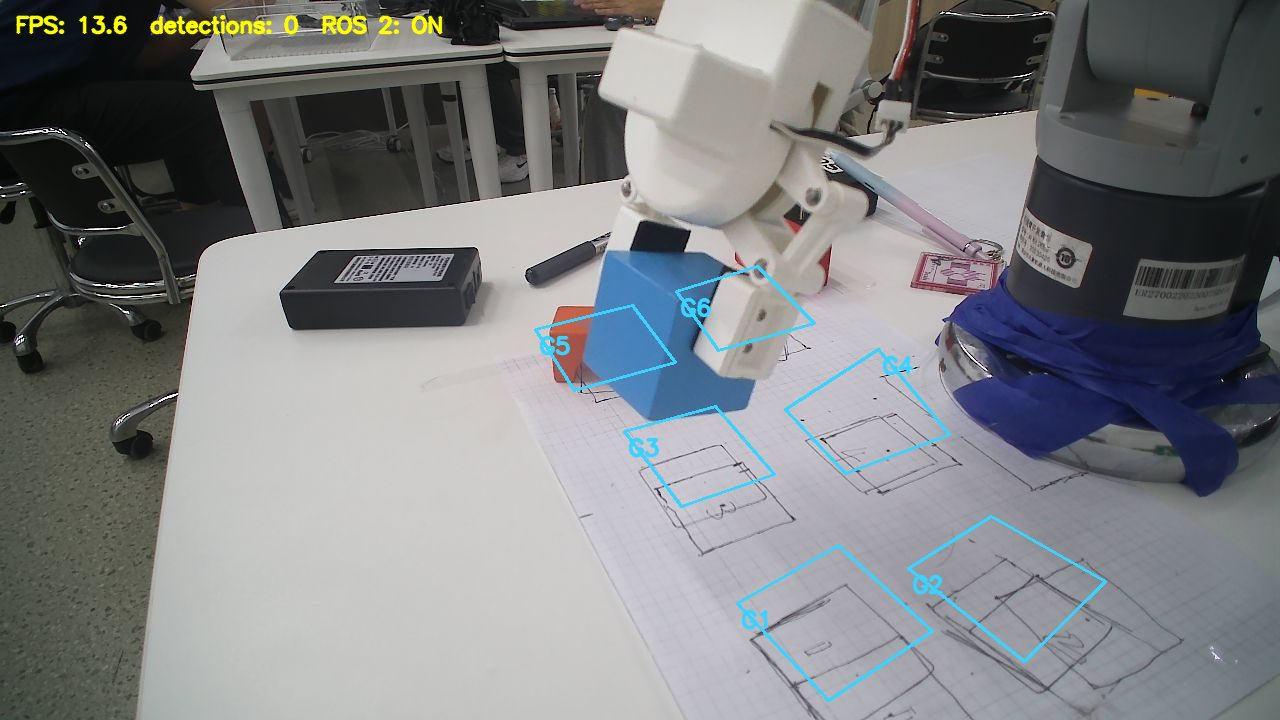
\includegraphics[width=\linewidth]{figures/lift.jpg}
\caption{Lift the object.}
\end{subfigure}
\caption{Physical motion stages shown in the supplied defense slides. These images illustrate the sequence; they do not provide a measured success rate.\src{defense}}
\label{fig:motion-stages}
\end{figure}

\subsection{TCP checks and clearance}

Sending a target did not mean that the arm had reached it. Before closing, the program waited for the TCP to settle near the grasp point. It sent the grasp route once, then read feedback without repeatedly sending the same joint target. Two consecutive acceptable samples were required. This reduced the chance of closing while the old arm was still moving.\src{motion}

\begin{table}[H]\tabstart
\caption{Selected motion acceptance settings, not measured positioning accuracy}
\begin{tabularx}{\textwidth}{@{}L{4.35cm}Y@{}}
\toprule Check & Configured condition\\\midrule
Ordinary grasp point & TCP horizontal error $\leq4$ mm; vertical error $\leq3$ mm.\\
Manually corrected grasp point & TCP horizontal error $\leq5$ mm; vertical error $\leq8$ mm.\\
Grasp stability & Two consecutive valid samples; up to nine checks at 0.75 s intervals.\\
Grasp joint guard & Other joint errors $\leq3^{\circ}$; joint 5 error $\leq8^{\circ}$.\\
Generated destination approach & Minimum clearance 50 mm; target 65 mm, also considering the highest recorded TCP position.\\
Post-release retreat & Measured TCP lift at least 75 mm, with a 0.5 mm feedback allowance.\\
\bottomrule
\end{tabularx}
\end{table}

The final code also adjusted difficult cells. It raised the requested grasp positions for grids 3 and 6 by 7 mm and 10 mm along their taught paths, and extended the grid 3 approach by 20 mm. These were generated targets, checked again through feedback. Since joint and Cartesian motion are not identical, the requested height change alone did not prove the physical result.\src{motion}

At the destination, the code could extend the taught release-to-approach direction to create a higher transition. After release, it checked the actual TCP height gain before returning across the workspace. These checks addressed low approach poses and the risk of touching the released object during departure. They still required a clear route and did not replace full obstacle detection.\src{motion}

\subsection{Class-specific gripping and delayed feedback}

One closing setting was not suitable for both object groups. The saved profile used OPEN=100, cube CLOSE=69, other CLOSE=40, and speed=20. These values use the gripper's control scale from 0 to 100; they are not angles or measured grip forces. The loader checked that the two close values were below the open value and that the profile was complete.\src{gripper}

The old gripper could respond late or stop briefly before reaching its final position. The program therefore checked visible feedback movement and several stable readings. For cube closing, the normal accepted feedback range was 64--72. A value of 73 was accepted only through a longer stable-contact check, requiring eight stable samples and enough closing movement. A brief pause at a more open position did not pass this check.\src{motion,gripper}

After lifting and before transfer, the program read the gripper position again without sending another close command. If an actuation failed, it could clear old commands and rebuild the control connection, with at most three sessions. Continued failure stopped the sequence. Position feedback was useful, but it could not measure grip force or prove that every object remained secure.\src{motion,gripper}

\subsection{Optional direction compensation}

An additional tool supported direction-based joint correction. For a joint approaching a pose from increasing or decreasing angles, it selected a matching correction and formed $q_{\mathrm{cmd},j}=q_{\mathrm{taught},j}+c_{j,d}$. This addressed the possibility that joint play and load caused different errors for different approach directions. When a joint target did not change, the previous direction was retained.\src{compensation}

The tool required validated settings, limited each correction to $3^{\circ}$, and supported a small preload movement. However, the supplied formal ROS worker did not enable this optional configuration by default. The main physical method was the corrected 17-pose route with feedback checks; the existence of the compensation tool does not establish a measured improvement in accuracy.\src{motion,compensation}
